\subsection{Formulación del problema}

En esta sección, estudiaremos el problema desde un punto de vista teórico, tomando el potencial de Pauli definido según \eqref{eq:def_int_pauli} y obteniendo sus propiedades analíticas para el caso de 2 partículas moviéndose en una única dimensión.

\subsubsection{Características generales}

En su forma más genera, un Hamiltoniano interactuando con un potencial dependiente de momentos tendrá ecuaciones de movimiento

\begin{align*}
\dot{\mathbf{q}}_i &= \dpart{H}{\mathbf{p}_i} = \frac{\mathbf{p}_i}{m} + \dpart{V_P}{\mathbf{p}_i} \equiv \frac{\mathbf{p}_i}{m} - \sum_{j\neq i} \mathbf{G}_{ij} \\
\dot{\mathbf{p}}_i &= -\dpart{H}{\mathbf{q}_i} = -\dpart{V_P}{\mathbf{p}_i} \equiv \sum_{j\neq i} \mathbf{F}_{ij}
\end{align*}

donde definimos las \textit{güerzas} $\mathbf{G}$ análogamente a las fuerzas habituales $\mathbf{F}$.
Para el potencial de Pauli, las güerzas cumplen $\mathbf{G}_{ij} = -\mathbf{G}_{ji}$ al igual que las fuerzas dado que $V_P$ depende de $\mathbf{p}_i - \mathbf{p}_j$ y toman la forma

\begin{align*}
\sum_{j\neq i} \mathbf{F}_{ij} &= -D \sum_{i<j} \left(-\frac{1}{2}\right)\dpart{s_{ij}^2}{\mathbf{q}_i}e^{-\frac{1}{2}s_{ij}^2} = D \sum_{i\neq j} \frac{\mathbf{q}_i - \mathbf{q}_j}{q_o^2}e^{-\frac{1}{2}s_{ij}^2} \Longrightarrow \mathbf{F}_{ij} = (\mathbf{q}_i - \mathbf{q}_j)\frac{D}{q_o^2}e^{-\frac{1}{2}s_{ij}^2} \\
\sum_{j\neq i} \mathbf{G}_{ij} &= -D \sum_{i<j} \left(-\frac{1}{2}\right)\dpart{s_{ij}^2}{\mathbf{p}_i}e^{-\frac{1}{2}s_{ij}^2} = D \sum_{i\neq j} \frac{\mathbf{p}_i - \mathbf{p}_j}{p_o^2}e^{-\frac{1}{2}s_{ij}^2} \Longrightarrow \mathbf{G}_{ij} = (\mathbf{p}_i - \mathbf{p}_j)\frac{D}{p_o^2}e^{-\frac{1}{2}s_{ij}^2}
\end{align*}

Según lo esperado, dada la simetría entre $p$ y $q$ en $V_P$, las expresiones resultan completamente análogas frente al intercambio $\mathbf{q}\leftrightarrow\mathbf{p}$. 
En nuestro caso particular de choque unidimensional, el Hamiltoniano toma la forma simplificada
\[ H(q_1, p_1; q_2, p_2) = \frac{1}{2m}\left( p_1^2 +p_2^2\right) + De^{-\frac{1}{2}\left(\frac{(p_1-p_2)^2}{p_o^2} + \frac{(q_1 - q_2)^2}{q_o^2}\right)} \]
pero esta expresión puede simplificarse aún más mediante el cambio de variables $x = x_1 - x_2$, $X = x_1 + x_2$ (donde $x$ se reemplaza $q$ o $p$ según corresponda), aprovechando que el hamiltoneano no depende de $Q$.
\begin{equation}{\label{eq:hamiltoniano_1D}}
H(q, p; P) = \frac{P^2}{4m} +\frac{p^2}{4m} + De^{-\frac{1}{2}\left(\frac{p^2}{p_o^2} + \frac{q^2}{q_o^2}\right)}
\end{equation}
donde el impulso total $P$ se conserva al ser nula la suma de fuerzas (acción y reacción sigue valiendo) y por lo tanto es una constante determinada por las condiciones iniciales del sistema.
Al ser el hamiltoneano definido a menos de una constante, podemos simplemente descartar el término $P^2/2m$ y continuar nuestro análisis.

Estas nuevas variables resultan más apropiadas, dado que en ellas resultará más clara la existencia (o no) de una región excluida dentro del espacio de fases.
Si el potencial emula bien el Principio de Exclusión de Pauli, deberiamos observar que $q$ y $p$ no pueden anularse simultaneamente. 

Es importante aclarar que el cambio de coordenadas $(q_1,q_2;p_1,p_2)\rightarrow (q,Q;p,P)$ así definida no resulta una transformación canónica pues no preserva los corchetes de Poisson originales $\poisson{q_i}{q_j} = 0 = \poisson{p_i}{p_j}$ y $\poisson{q_i}{p_j} = \delta_{ij}$
\begin{align*}
\poisson{q}{Q} &= \poisson{q_1-q_2}{q_1+q_2} =  \poisson{q_1}{q_2} + \poisson{-q_2}{q_1} = 0 \\
\poisson{p}{P} &= \poisson{p_1-p_2}{p_1+p_2} = \poisson{p_1}{p_2} + \poisson{-p_2}{p_1} = 0 \\
\poisson{q}{p} &= \poisson{q_1-q_2}{p_1-p_2} =  \poisson{q_1}{p_1} + \poisson{-q_2}{-p_2} = 2 \\
\poisson{Q}{P} &= \poisson{q_1+q_2}{p_1+p_2} =  \poisson{q_1}{p_1} + \poisson{q_2}{p_2} = 2 \\
\poisson{q}{P} &= \poisson{q_1-q_2}{p_1+p_2} = \poisson{q_1}{p_1} + \poisson{-q_2}{p_2} = 1 - 1 = 0 \\
\poisson{q}{P} &= \poisson{q_1+q_2}{p_1-p_2} = \poisson{q_1}{p_1} + \poisson{q_2}{-p_2} = 1 - 1 = 0
\end{align*}

A pesar de que resulta sencillo corregir esto dividiendo las nuevas variables por $\sqrt{2}$, no nos interesa particularmente que las nuevas variables sigan las ecuaciones de Hamilton, dado que no pretendemos integrarlas. Volveremos sobre esto en la sección \textbf{\ref{sec:teo_fases}}.


\subsubsection{Adimensionalización}

El Hamiltoniano definido por \eqref{eq:hamiltoniano_1D} dispone de 4 parámetros $m, q_o, p_o, D$ que determinarán su comportamiento cualitativo.
Sin embargo, puede apreciarse que las constantes de $q_o$ y $p_o$ claramente resultan meros factores de escala de la interacción y probablemente no jueguen ningún rol en la forma funcional de los observables del sistema.
Pero no solo $q_o$ y $p_o$ son irrelevantes, dado que usando el teorema $\Pi$, podemos redefinir variables para eliminar un tercer parámetro adicional. 
Elegimos la masa $m$ como el tercer parámetro a eliminar y , de esta manera, redefinimos $q$, $p$ y $H$ según
\begin{equation}{\label{eq:unidades_red}}
q^* = q/q_o \qquad p^* = p/p_o \qquad H^* = Hm/p_o^2
\end{equation}
de manera que el nuevo Hamiltoniano reducido resulte 

\begin{equation}{\label{eq:ham_red_1d}}
H^*(q^*, p^*) = \frac{p^{*2}}{4} + \frac{Dm}{p_o^2}e^{-\frac{1}{2}(q^{*2}+p^{*2})} \equiv \frac{p^{*2}}{4} + D^* e^{-\frac{1}{2}(q^{*2}+p^{*2})}
\end{equation}
donde queda en evidencia el rol de $D^* = Dm/p_o^2$ como único parámetro funcional del problema.
Claramente, para el caso $D^*\to 0$ recuperamos un hamiltoneano de partícula libre, cuyo espacio de fases es bien conocido.
Por otro lado, para el caso $D^*\to \infty$, el término cinético $p^2/4$ resulta despreciable y tenemos un Hamiltoniano dominado puramente por el potencial de Pauli, cuya simetría es esférica en el espacio de fases.

En general, cualquier observable reducido $O^*$ del sistema tendrá una dependencia únicamente de $D^*$ ($O^* = O^*(D^*)$).
Es importante aclarar que esta adimensionalización puede aplicarse igualmente a sistemas con más de 2 partículas, razón por la cual utilizaremos este resultado a continuación y a lo largo de todo este trabajo.


\subsubsection{Espacio de fases}{\label{sec:teo_fases}}

Ahora si, atacaremos el Hamiltoniano reducido de \eqref{eq:ham_red_1d} con el objetivo de obtener el espacio de fases.
En nuestro caso, teniendo dos solo coordenadas $(q^*,p^*)$, esto consiste en obtener las curvas $q^*(p^*)$ o $p^*(q^*)$ a través de las ecuaciones de Hamilton.

Sin embargo, como dijimos, las ecuaciones de Hamilton para $(q^*,p^*)$ no se preservan, pero esto no es un problema.
Independientemente de la transformación, es un hecho que el Hamiltoniano se conserva.
Por lo tanto, podemos simplemente plantear la conservación de $H^*(q^*,p^*)\equiv E^*$ para obtener las curvas de nivel de $H^*(q^*,p^*)$.
Claramente, la opción más económica es despejar $q^*(p^*)$ como
\begin{equation}{\label{eq:qvsp}}
q^{*2}(p^*) = -p^{*2} - 2 \log\left( \frac{E^*-p^{*2}/4}{D^*} \right) \equiv -p^{*2} - 2 \log\left( \frac{p_\infty^2-p^{*2}}{4D^*} \right)
\end{equation}
donde usamos que $E^* = p_\infty^{*2}/4$ para $q\to\infty$ y así reescribir intuitivamente la dependencia.
Justamente, tenemos consistentemente $q^{*2}(p^*\to\pm p_\infty) = \infty$. 
En particular, esto implica que la curva está acotada para $-p_\infty \leq p^* \leq p_\infty$ mientras que $q^*$ resulta a priori no acotado.

Como podriamos haber intuído, las curvas de nivel \eqref{eq:qvsp} son invariantes ante reflexiones en $q$ y/o $p$, por lo que nos basta con analizar el caso $q^*\geq 0$, obteniendo la otra mitad del diagrama de fases por reflexión. 

Dado que planteamos este potencial con el objetivo de obtener una región excluida alrededor del $(q,p)=(0,0)$, resulta natural analizar la curva $(q^*,p^*)$ que pasa por el $(0,0)$.
Para esta curva, debe ser $E^* = H^*(0,0) = D^*$ y 
\[ q^{*2} = -p^{*2} - 2\log\left( \frac{4D^*-p^{*2}}{4D^*} \right) 
= -p^{*2} - 2\log\left( 1-\frac{p^{*2}}{4D^*} \right) \]

Para que esta curva que pasa por el $(0,0)$ exista, deben existir $(q^*, p^*)$ arbitrariamente cerca.
Para este $p^*$, expandimos en serie de Taylor truncada
\[ q^{*2} = -p^{*2} - 2\log\left( 1-\frac{p^{*2}}{4D^*} \right) \approx -p^{*2} + 2\frac{p^{*2}}{4D^*}  = p^{*2} \left( \frac{1}{2D^*} -1 \right) \geq 0 \Longleftrightarrow D^* \leq \frac{1}{2} \]

Por lo tanto, si $D^*\leq 1/2$, existe una curva de nivel de $H^*$ que pasa por el $(0,0)$ y, por lo visto en \ref{eq:qvsp}, alcanza $(\infty, \pm p_\infty)$.
En caso contrario, la curva de nivel de $H^*= D^*$ consiste únicamente del punto $(0,0)$ y efectivamente existe una exclusión, una zona inaccesible.

Planteado esto, el próximo paso consiste en analizar la forma de las curvas de nivel $q^{*2}(p^*)$.
Realizamos entonces un estudio de función, comenzando por los extremos de $q^{*2}(p^*)$
\[ 0 = \dpart{q^{*2}}{p^*} = -2p^* - 2\frac{-2p^*}{p_\infty^2-p^{*2}} 
= \frac{-2p^*}{p_\infty^2-p^{*2}} \left( p_\infty^2-p^{*2} - 2 \right) \Leftrightarrow p^{*2} = p_\infty^2 - 2 \quad \text{ o } \quad p^* = 0 \]

Nuevamente, vemos que estos extremos son simétricos respecto de $p^*=0$. 
Sin embargo, es más interesante notar que si $p_\infty^2 > 2$ o $E^* > 1/2$ existen 3 extremos.
En caso contrario, solo existe uno.

Para el caso $E^* > 1/2$, dado que $q^*$ viene desde el infinito en $\pm p_\infty$, es necesario que los extremos $p^{*2} = p_\infty^2 - 2$ sean mínimos y, por simetría, el extremo $p^*=0$ debe ser un máximo. Por otro lado, para el caso $E^*\leq 1/2$ solo tenemos un único extremo en $p^*=0$, que necesariamente debe ser un mínimo. 

Esquematicamente, tenemos entonces 2 tipos de curva, aquellas con dos mínimos (para $E^* > 1/2$) y aquellas con un mínimo (para $E^* \leq 1/2$).
Esto, sin embargo, no está completo dado que aún no confirmamos que $q^{*2}\geq 0$ en los mínimos.

\[ q^{*2}(p^*=0) = -2\log \left( \frac{p_\infty^2}{4D^*} \right) = 2\log \left( \frac{D^*}{E^*} \right) \geq 0 \Leftrightarrow E^*\leq D^* \]
\[ q^{*2}(p^{*2}=p^2_\infty-2) = 2-p_\infty^2 -2\log \left( \frac{2}{4D^*} \right) = 2 - p_\infty^2 + 2\log \left( 2D^* \right) \geq 0 \Leftrightarrow E^*\leq \frac{1}{2}\left( 1 + \log(2D^*) \right)  \]

Tenemos entonces dos cotas para $E^*$ que, llamativamente, coinciden para el caso $D^*=1/2$. 
Esto no es casual, dado que analizando ambas funciones vemos que para $D^*\geq1/2$ la segunda cota resulta estrictamente más fuerte que la primera.
Es más, si recordamos que la segunda cota solo tiene sentido para $E^*>1/2$ reobtenemos
\[ \frac{1}{2} ( 1 + \log(2D^*) ) > \frac{1}{2} \Longleftrightarrow D^* > \frac{1}{2} \]

Por lo tanto, la existencia de ambos mínimos positivos ($E^*>1/2$ y $q^{*2}(p^{*2}=p^2_\infty-2)\geq 0$) se da si y solo si existe un área excluida ($D^*>1/2$).
Dado que son condiciones equivalentes, asumamos $D^*>1/2$ y analicemos las curvas de nivel obtenidas.

En particular, existe un valor de energía crítica $E^*_c = (1+\log(2D^*))/2$ para la cual $q^{*2}(p^{*2}=p^2_\infty-2) = 0$. 
Esto implica $q^*(p^{*2}=p^2_\infty-2)=0$ y, por lo tanto, tenemos una curva que conecta $(\infty, \pm p_\infty)$ con $(0,p^2_\infty-2)$.
Por simetría de reflexión en $q$, tenemos una curva idéntica que conecta $(-\infty, \pm p_\infty)$ con $(0,p^2_\infty-2)$ y, por lo tanto, una única curva que conecta $(-\infty, \pm p_\infty)$ con $(\infty, \pm p_\infty)$.
Esto también es válido $\forall$ $E^*\geq E^*_c$, dado que si $q^{*2}(p^{*2}=p_\infty^2-2)\leq 0$ y $q^{*2}(p^{*2}=p_\infty^2)\geq 0$, por continuidad debe existir un $p_\infty^2-2\leq p^*_c\leq p_\infty^2$  tal que $q^{*2}(p^*_c) = 0$ y el argumento anterior aplica de forma idéntica.
Físicamente, esto corresponde al caso en que las partículas comienzan acercándose desde el infinito y se atraviesan, alejándose infinitamente de nuevo. 

Sin embargo, para $E^*\leq E^*_c$, tenemos $q^{*2}(p^*) > 0$  $\forall$ $p^*$ (dado que el mínimo es estrictamente positivo).
Este caso, por el contrario, corresponde a un rebote en el que las partículas se acercan hasta una distancia mínima para luego ser repelidas de nuevo hasta el infinito. 
Es interesante notar, sin embargo, que esta distancia mínima se alcanza dos veces, por lo que las particulas se acercan desde el infinito hasta una distancia mínima, se alejan una distancia finita, vuelven a acercarse a la distancia mínima y finalmente se alejan hasta el infinito.

Para el caso $D^*\leq 1/2$, inevitablemente tenemos un solo mínimo en $p^*=0$ que resulta positivo si y solo si $E^*\leq D^*$. 
En el caso particular $D^*=E^*$ tenemos una curva de nivel que viene desde $(\infty,\pm p_\infty)$ y llega hasta $(0,0)$ como habíamos visto previamente.
Por lo tanto, tenemos curvas cóncavas cuyo mínimo tiende a $0$ a medida que $E^*$ tiende a $D^*$.
Este caso corresponde nuevamente a un rebote.
A diferencia del caso $D^*>1/2$, este caso corresponde a un rebote clásico: las partículas se acercan desde el infinito hasta una distancia mínima y luego se alejan infinitamente.

Para $E^*>D^*$ tenemos que $q^{*2}(0) < 0$ y $q^{*2}(p^{*2}=p_\infty^2)\geq 0$. 
Análogamente a lo anterior, por continuidad debe existir $0\leq p^*_c\leq p_\infty^2$ tal que $q^{*2}(p^*_c) = 0$ y nuevamente tenemos una curva que conecta $(-\infty, \pm p_\infty)$ con $(\infty, \pm p_\infty)$. 

En resumen, tenemos 4 casos que dan origen a 3 curvas distintas (ver \textbf{Tabla TABLA}).
Estas curvas y sus diferencias pueden apreciarse en \textbf{Figura CURVAS}.

\begin{table}[h]
	\centering
	\begin{tabular}{|c|c||c|c|}
		\hline
		\multicolumn{2}{|c||}{$D^*\leq1/2$} & \multicolumn{2}{c|}{$D^*>1/2$} \\ \hline
		    $\qquad E^*\leq D^* \qquad$      &    $\qquad E^*> D^* \qquad$       &    $E^*>\frac{1}{2}(1+\log(2D^*))$        &    $E^*\leq\frac{1}{2}(1+\log(2D^*))$     \\ \hline
		    \textbf{Rebote simple}      &    \multicolumn{2}{c|}{\textbf{Atraviese}}     &     \textbf{Rebote doble}    \\ \hline
	\end{tabular}
\end{table}

La existencia de región excluida existe solo para $D^*>1/2$ puede apreciarse para las curvas de doble rebote, que parecen estar circunventando el origen. 
Como dijimos, a medida que $E^*\to E^*_c = (1+\log(2D^*))/2$ estas curvas acercarán sus mínimos al eje $q^*=0$ hasta transformarse en curvas de atraviese.
Es justamente para $E^*\to E^*_c $ por debajo donde los mínimos de $q\geq0$ y $q\leq0$ se conectan, encerrando la región excluída. 
Por lo tanto, la curva $q^{*2}(p^*; E^*=E_c^*)$ define el perímetro de esta región y podemos utilizarla para calcular el área total encerrada según

\begin{align*}
A^* = 2\int_{-\sqrt{p_\infty^2-2}}^{\sqrt{p_\infty^2-2}} q^*(p) dp \Bigg|_{p_\infty^2=4E^*_c}
&= 4\int_{0}^{\sqrt{p_\infty^2-2}} \sqrt{-p^2 - 2\log\left( \frac{p_\infty^2-p^2}{2} + \log(2D^*) \right)} dp \Bigg|_{p_\infty^2=4E^*_c}
\end{align*}

Mediante el cambio de variables $x = (p_\infty^2-p^2)/2$, $dx = -p dp \Rightarrow dp = -dx/\sqrt{p_\infty^2-2x}$ y usando que $p_\infty^2 = 4E^*_c$ y $\log(2D^*) = 2E_c^* - 1$

\begin{equation}{\label{eq:area_int_ex}}
A^* = 4\int_{1}^{2E_c^*} \frac{\sqrt{-4E_c^* + 2x - 2\log(x) + 4E_c^* - 2}}{\sqrt{4E_c^* - 2x}} dx
= 4\int_{1}^{2E_c^*} \frac{\sqrt{x -1 - \log(x)}}{\sqrt{2E_c^* - x}} dx
\end{equation}
donde debemos recordar que $2E_c^* = 1 + \log(2D^*) $ y que $A^*$ es el área reducida, siendo el área total $A = q_op_oA^*$.

Sin embargo, la integral de \eqref{eq:area_int_ex} no puede expresarse como una combinación de funciones conocidas, lo cual nos impide por completo obtener una forma funcional clara.
Aún así, podemos realizar una integración numérica de $A^*$ vía regla de trapecios.
Debemos tener especial cuidado en el extremo superior, donde el integrando diverge.
El resultado de esta integración numérica en un amplio rango de $D^*$ puede apreciarse en la \textbf{Figura AvsD TEO}, donde vemos que rápidamente se alcanza una tendencia lineal $A \approx \alpha \log(D^*) + \beta$.

\begin{figure}
%	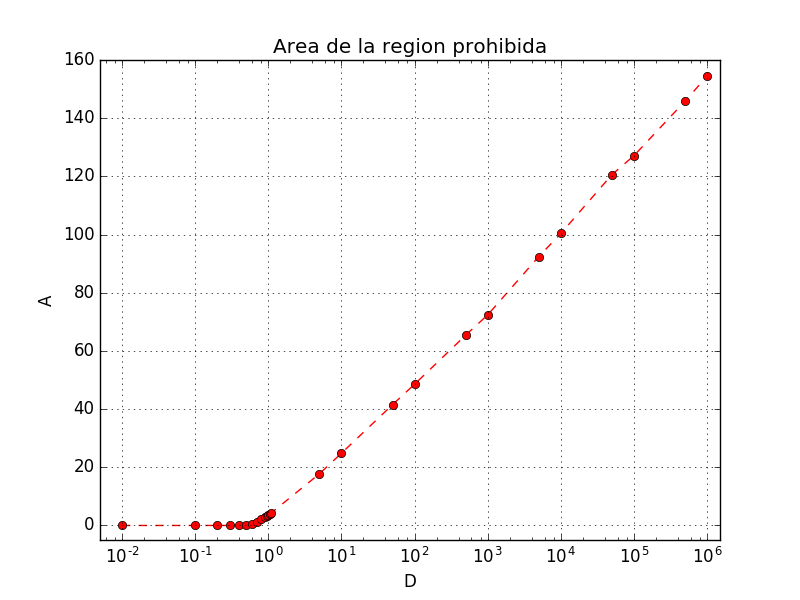
\includegraphics[contenidos...]{choque1d/AvsD}
\end{figure}

Más adelante retomaremos este análisis del espacio de fases desde un punto de vista computacional, simulando el choque y confirmando nuestros resultados con esta sección.




\subsection{Integradores y simplecticidad}

Como dijimos, las curvas $q(p)$ del diagrama de fases mantienen el Hamiltoneano $H(q,p)$ constante.
A la hora de simular, un método que conserve la energía del sistema arrojará estas curvas $q(p)$ inmediatamente.

Una simulación de dinámica molecular evolucionando el sistema con las ecuaciones de Hamilton con un integrador simpléctico nos asegura esto más, por lo que resulta mucho más natural que otros métodos donde la energía fluctua (como Metropolis-Montecarlo).

\subsubsection{Implementación de integradores}

Según lo que discutimos en la sección \ref{sec:int_simpl}, dado que el Hamiltoniano \eqref{eq:hamiltoniano_1D} es no separable, no disponemos de integradores simplécticos y explícitos.
Con el objetivo de comparar, decidimos implementar 2 integradores no simplécticos pero explícitos y un integrador simpléctico pero no explícito.

Además, para simplificar la notación definimos \[y = \binom{p}{q} \qquad J = \begin{pmatrix}
0 & \mathbb{I} \\
-\mathbb{I} & 0
\end{pmatrix}
\]

Los integradores implementados son Euler, un Runge-Kutta de orden 2 (RK2) y MidPoint Rule (MPR).
Los esquemas pueden apreciarse junto con su información relevante en la \textbf{Tabla \ref{tab:integradores}}. 
La simplecticidad de MPR fue probada en \ref{sec:int_simpl} mientras que la no simplecticidad de Euler y RK2 se encuentra en el apéndice \ref{sec:no_simp}.

\begin{table}[h]
	\centering
	\begin{tabular}{|c|c|c|c|c|}
		\hline
		\textbf{Integrador} & \textbf{Esquema} & \textbf{Orden} & \textbf{¿Explícito?} & \textbf{¿Simpléctico?} \\ \hline
		Euler & $ y_{n+1} = y_n + hJ^{-1}\nabla H(y_n)$ & $1$ & Si & No \\ \hline
		Runge-Kutta 2 & $y_{n+1} = y_n + hJ^{-1}\nabla H\left(y_n+\frac{h}{2}\nabla H(y_n) \right)$ & $2$ & Si & No \\ \hline
		Midpoint Rule & $y_{n+1} = y_n +  hJ^{-1}\nabla H\left(\frac{y_n+y_{n+1}}{2} \right)$ & $2$ & No & Si \\ \hline
	\end{tabular}
	\caption{Comparación de los integradores utilizados}
	\label{tab:integradores}
\end{table}

Dado que no es explícito, para el integrador MPR implementamos además un método de punto fijo para poder resolver cada paso.
Sumando $y_n$ a cada lado del esquema MPR y dividiendo por 2, podemos redefinir $Z = \frac{y_n+y_{n+1}}{2}$ tal que
\[ Z = y_n + \frac{h}{2}J\nabla H(Z) \equiv F(Z) \]
y resolver esta ecuación de punto fijo con parámetro conocido $\mathbf{y}_n$ en \textit{cada iteración} evaluando múltiples veces $F(Z)$.
En principio, puede probarse que $|DF(Z)|<1$ (punto fijo converge) para $h$ suficientemente chico dado que el Hessiano del potencial de Pauli está acotado (es gaussiano).
Sin embargo, la cota para $h$ dependerá de los parámetros $p_o$, $q_o$ y $D$ e incluso podría depender del número de partículas $N$ del sistema.
Por lo tanto, en principio nos conformaremos con saber que tal $h$ existe e intentar encontrarlo según la situación.
En lo que sigue, siempre resolvimos el problema de punto fijo $Z = F(Z)$ utilizando 5 iteraciones, al notar que valores más altos no mejoraban apreciablemente la convergencia.

\subsubsection{Conservación de la energía}

\subsubsection{Teorema de Liouville y volumen de fases}


\subsection{Estudio numérico del espacio de fases}
